% =====================================================================
%  AY27 RSE RENEWAL PROPOSAL  --  SPECFEM++  (2027-2029)
%  PI: Jeroen Tromp (sole PI).  2 RSEs x 2 years, 30% RC co-funding.
%  DRAFT -- language/style modeled on the funded 2024 RSE proposal.
%  Flags: \note{...} marks open items / numbers to verify before submit.
%  Narrative limit: 3 pages (references excluded) + 1-page budget + PI CV.
% =====================================================================
\documentclass[11pt,letter]{article}
\usepackage[top=1in, bottom=1in, left=1in, right=1in]{geometry}
\usepackage{times}
\usepackage[english]{babel}
\usepackage[linkcolor=black,colorlinks=true,linkcolor=Blue,citecolor=Maroon, urlcolor=gray]{hyperref}
\urlstyle{same}
\usepackage{enumitem}
\usepackage{amsmath}
\usepackage{amssymb}
\usepackage{mathrsfs}
\usepackage{graphicx}
\usepackage{float}
\usepackage{subcaption}
\captionsetup{
    width=0.95\textwidth,
    labelfont=bf,
    font={small,it},
}
\usepackage{natbib}
\usepackage[usenames,dvipsnames]{color}
\usepackage{wrapfig}
\graphicspath{{figures/}}

\usepackage{tikz}
\newcommand{\ExternalLink}{%
    \tikz[x=1.2ex, y=1.2ex, baseline=-0.05ex]{%
        \begin{scope}[x=1ex, y=1ex]
            \clip (-0.1,-0.1)
                --++ (-0, 1.2) --++ (0.6, 0) --++ (0, -0.6)
                --++ (0.6, 0) --++ (0, -1);
            \path[draw, line width = 0.5, rounded corners=0.5]
                (0,0) rectangle (1,1);
        \end{scope}
        \path[draw, line width = 0.5] (0.5, 0.5) -- (1, 1);
        \path[draw, line width = 0.5] (0.6, 1) -- (1, 1) -- (1, 0.6);
        }
    }

\usepackage{mycommands}
\usepackage{shorthands}

% --- draft-only flag for open items / numbers to verify ---------------
\newcommand{\note}[1]{\textbf{\textcolor{Red}{[#1]}}}

% tighten section spacing to help fit 3 pages
\usepackage{titlesec}
\titlespacing\section{0pt}{6pt plus 2pt minus 2pt}{2pt plus 1pt minus 1pt}
\titlespacing\subsection{0pt}{4pt plus 2pt minus 2pt}{1pt}

\widowpenalty10000
\clubpenalty10000

\begin{document}

\noindent {\large{\textbf{SPECFEM++: Sustaining and Extending a Performance-Portable Spectral-Element Library for Wave Propagation Modeling and Imaging}}}
\vspace{-0.4em}\newline
\noindent {\small PI: Jeroen Tromp \quad\textbullet\quad RSE Renewal (AY27) \quad\textbullet\quad Two RSEs, two years (July 2027--June 2029)}
\vspace{-0.2em}\newline
\noindent\rule{\textwidth}{0.4pt}

\paragraph{Summary}
We request renewal of RSE co-funding to continue the development of \SFPP, the \software{Kokkos}/\software{C++} rewrite of the \SF\ software suite for simulating seismic wave propagation and performing adjoint tomography. Over the past two years, a three-RSE team transformed a single-developer proof-of-concept into a released, benchmarked, and community-adopted code that is on track to reach feature parity with \SFG\ by the start of this award. Where the previous award \emph{built the foundation}, this renewal \emph{uses it}: we will deliver science beyond the reach of legacy \SF---a frequency-domain solver---while hardening the production code and growing the community that will ultimately sustain it. We request 30\% university co-funding for two continuing RSEs for two years; the PI will provide the remaining 70\% \note{name Princeton match source---BLOCKING budget item}. The foundational build genuinely required three RSEs; that phase is complete, so this is a right-sized, two-RSE consolidation, not a retreat.

% =====================================================================
\section{Research Context}
% =====================================================================
Simulating how seismic waves propagate through the Earth underpins problems ranging from earthquake and exploration seismology to planetary science, helioseismology, non-destructive testing, and medical imaging. For a quarter-century the community's standard tool for this task has been the \SF\ suite (\href{https://specfem.org/}{specfem.org \ExternalLink}), an open-source code for forward modeling and adjoint tomography of 2D and 3D acoustic, (an)elastic, gravity, and ultrasound wave propagation. It accounts for attenuation, rotation, self-gravitation, bathymetry, topography, ellipticity, and fluid--solid interfaces, and it scales from laboratory to global problems.

The scientific frontier is now a coupled, planetary-scale ``Earth simulator'': a single framework in which seismic, ocean, and atmospheric wavefields interact with self-gravitation and rotation, and which can be \emph{inverted} with adjoint methods to image the planet at unprecedented resolution. This ambition is what sets \SFPP's requirements. \SFPP\ is the modern successor to the incumbent standard---a complete \software{C++}/\software{Kokkos} rewrite of \SFTWOD, \SFTHREED, and \SFG\ designed to carry the \SF\ community onto today's heterogeneous, exascale-class hardware and to express physics the original code cannot.

% =====================================================================
\section{Research Impact and Software Opportunity}
% =====================================================================
The impact of the software is exceptional and easy to quantify. Since its inception in 1999, over 230 publications have used \SF, its annual citations exceed 2{,}500 per year, and its software h-index is 84 (\href{https://scholar.google.com/citations?user=bvjzHdUAAAAJ}{Google Scholar \ExternalLink}); it is used across six application domains and has garnered more than 600 GitHub stars. This footprint is reinforced by the PI's own standing in the field \note{PI record: $\sim$30{,}500 citations, h-index 78---confirm/round for CV}.

Legacy \SF\ is written in \software{Fortran90} with separate \software{CUDA} and \software{OpenMP} paths, and this design cannot follow the science in two ways at once. First, it cannot ride modern heterogeneous hardware without maintaining divergent, architecture-specific codebases. \software{Kokkos}~\citep{Trott2022} resolves this: it is a \software{C++} performance-portability library that lets developers ``write once, run anywhere''---mapping a single implementation onto \software{CUDA}, \software{HIP}, \software{SYCL}, and \software{OpenMP} backends---so the team can focus on physics and algorithms rather than hardware. The approach is proven at Princeton: \software{Kokkos} ported the \software{Athena++} magnetohydrodynamics code to GPUs with performance matching the native \software{CUDA} implementation~\citep{Stone2020,Grete2021}. Second, the legacy architecture cannot readily express the new physics the field now needs. \SFPP's modern \software{C++} design removes both limits at once.

\emph{Feature parity with \SFG\ is the launch pad, not the goal.} Parity makes \SFPP\ an adoptable successor to the code the community already relies on, and it is on track to be reached by \note{$\sim$summer 2027}---the start of this award. The opportunity for 2027--2029 therefore lies \emph{beyond} legacy \SF: the modern architecture already enables physics the \software{Fortran} code could not (semi-discontinuous Galerkin methods, Cosserat media), and it opens the way to a frequency-domain solver and to the coupled Earth-simulator physics above. Domain scientists supply the physics; what turns it into performant, maintainable, community-usable software is professional research software engineering. That is the need this proposal addresses.

% =====================================================================
\section{Research Software Engineering}
% =====================================================================

This is professional software-engineering work, not a science postdoc's side project. It demands \software{Kokkos} performance portability, \software{C++} template metaprogramming (the mechanism by which \SFPP\ generates specialized, high-performance kernels at compile time while exposing a single interface), cross-architecture continuous integration, release engineering, and rigorous benchmarking---skills that are the core of the RSE profession and difficult to sustain through rotating students or postdocs.

The past two years proved that a \emph{coordinated team} with formal project management is equally essential. A single RSE could not have delivered the current code; a team working with issue tracking, code review, continuous integration, and a shared roadmap did. Just as important, the division of labor between the RSE manager and the PI has become crystal clear---there is never a question of who works on what, which lets the scientists set direction while the RSEs own execution. This working model is precisely what the RSE program exists to provide, and it is why delivery accelerated once the team was in place.

% =====================================================================
\section{Previous Results}
% =====================================================================
In the roughly 22 months since the two new RSEs were hired (November 2024), the team turned a single-developer proof-of-concept into a released, benchmarked, and community-adopted code---and pushed past the original plan.

\noindent\textbf{Delivered on plan.} 2D and 3D forward--adjoint solvers are in place; the code has reached roughly \note{80\%} parity toward \SFG\ and is on track for full parity by the award start. Six public releases (v0.1.0$\rightarrow$v0.6.0) have shipped at an accelerating cadence since the team formed~\citep{SPECFEMPP2026}.

\noindent\textbf{Performance.} Benchmarks (Fig.~\ref{fig:perf}) show the 2D solver is already \textbf{1.43--2.15$\times$ faster} than \SFTWOD\ on CPU and 1.08--1.58$\times$ faster on GPU; the 3D solver already runs at \textbf{$\sim$60\% of native \SFTHREED\ with no performance tuning}. Closing the remaining gap to parity is therefore a tractable engineering target, not a research risk.

\noindent\textbf{Beyond plan.} The flexible architecture has already enabled new science the legacy code could not support: a 2D semi-discontinuous Galerkin method~\citep{DG2026} and wave propagation in Cosserat (micropolar) media~\citep{Cosserat2026}, each the subject of a manuscript in preparation (and, for the former, a thesis chapter), with a reference benchmark already merged.

\noindent\textbf{Community traction.} The repository has grown to \note{61 stars / 22 forks}; the project received its first \emph{unprompted} external pull request before its two-year anniversary; and active users now include two undergraduates, one graduate student, and one postdoc. The team has run two developer hackathons to onboard new contributors to the codebase.

The lesson for this renewal is specific: the foundational build genuinely required a three-RSE team, and that phase is now done. The next two years are a disciplined, two-RSE consolidation and extension.

% =====================================================================
\section{Proposed Work and Deliverables}
% =====================================================================
With parity to \SFG\ reached at the award's start, the renewal shifts from catching up to legacy \SF\ to surpassing it. Work is organized around three primary deliverables for two RSEs over two years (Fig.~\ref{fig:gantt}).

\begin{figure}[!ht]
    \centering
    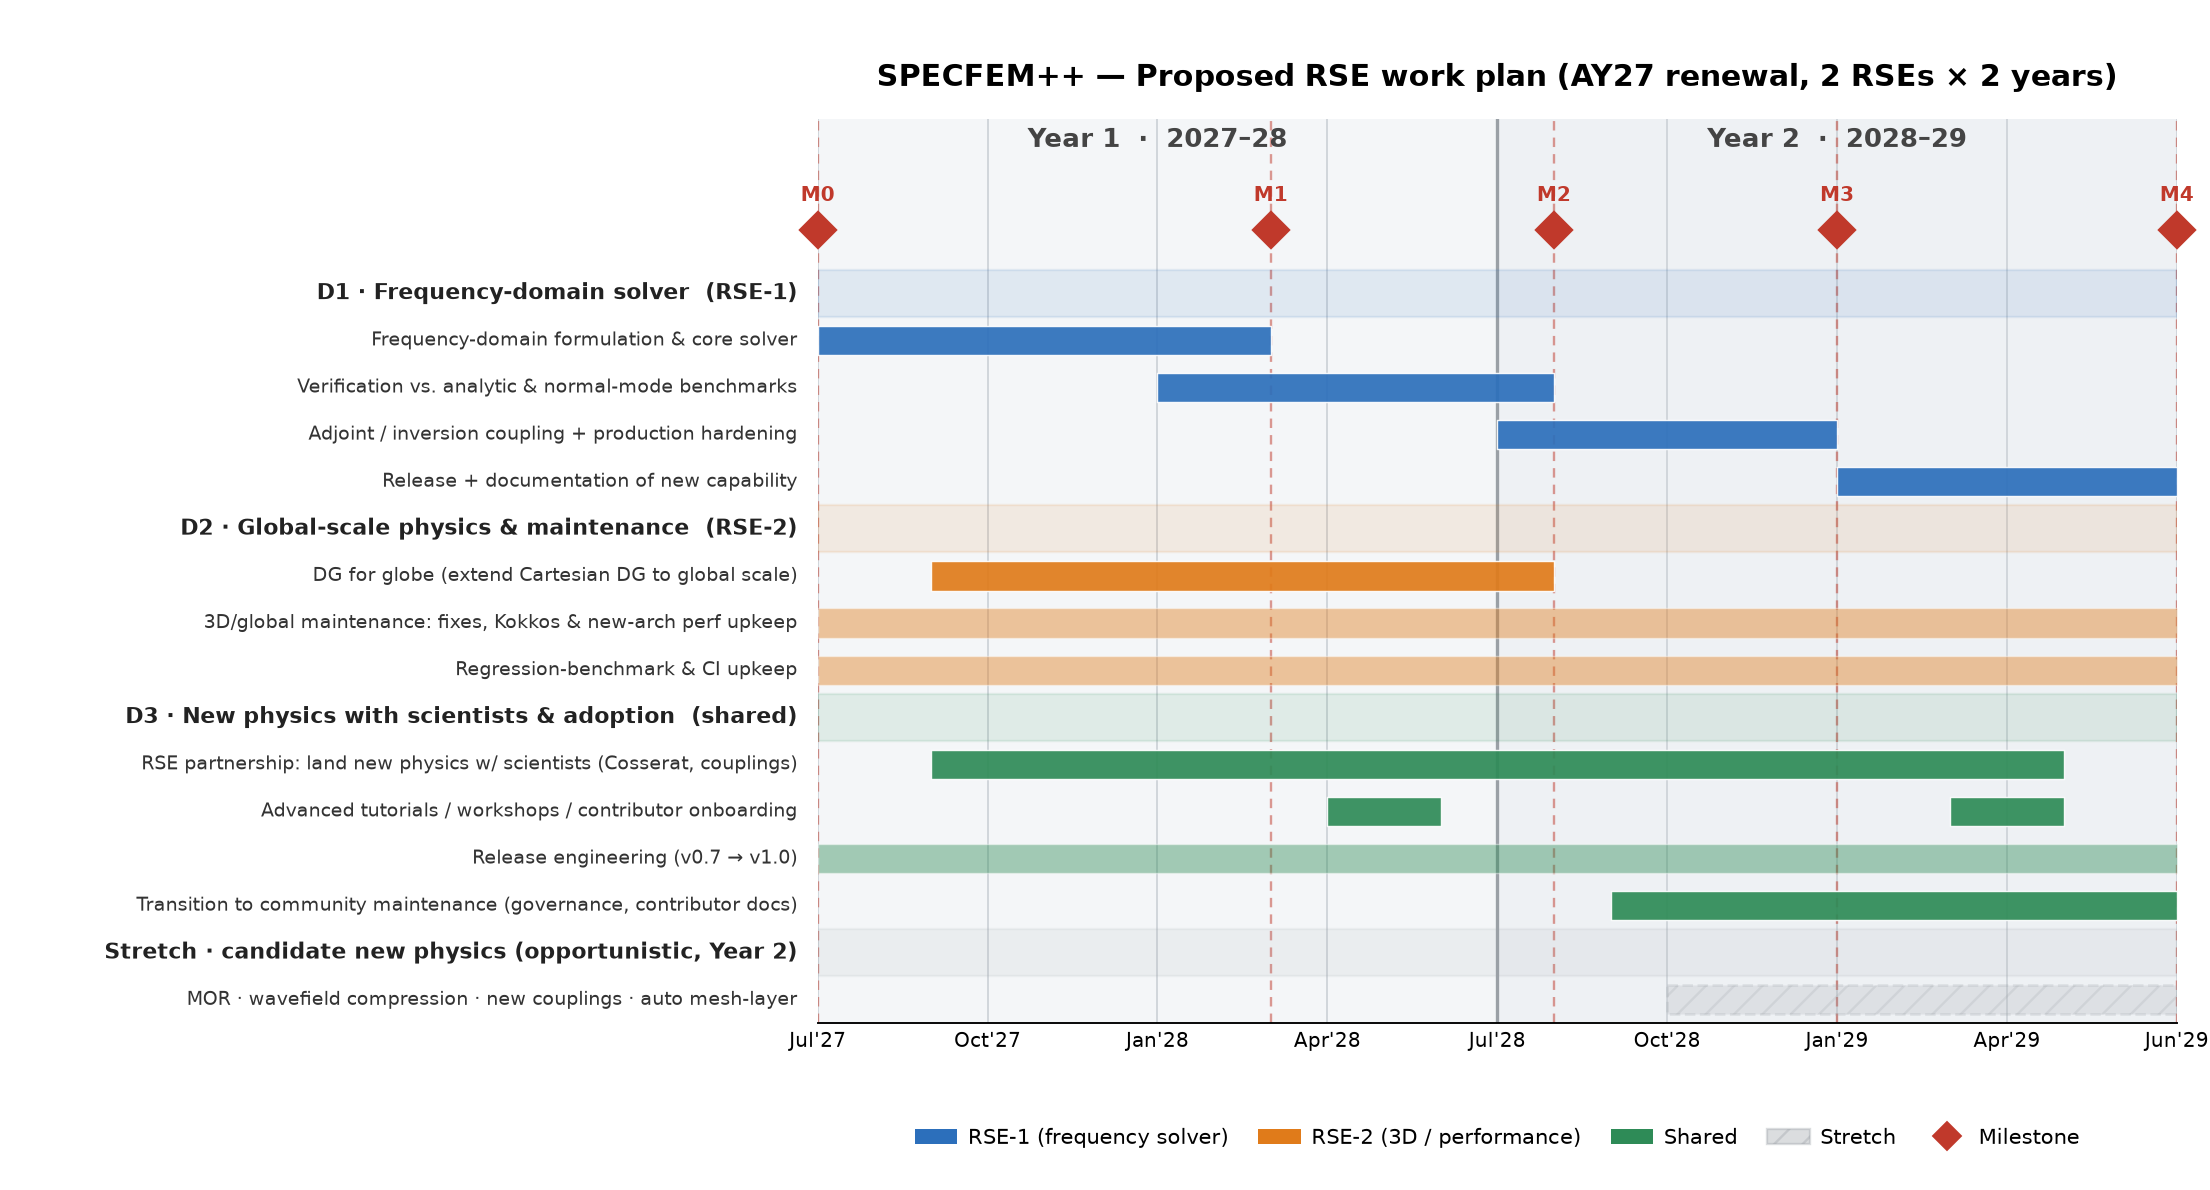
\includegraphics[width=0.98\textwidth]{proposed_gantt.png}
    \caption{Proposed two-year work plan (July 2027--June 2029). D1 (frequency-domain solver) is led by one RSE; D2 (global-scale physics and maintenance) by the other; D3 (new physics with scientists and adoption) is shared. Milestones M0--M4 align to release and capability completions; stretch items are opportunistic Year-2 targets.}
    \label{fig:gantt}
\end{figure}

\vspace{-0.4em}
\begin{description}[leftmargin=1.3em, itemsep=1pt, topsep=1pt]
\item[\textnormal{\textbf{D1 --- Frequency-domain solver (primary).}}] Build on the existing implicit/static-solver line (implicit Newmark time integration, \software{Belos}/\software{Trilinos} iterative solvers) toward a production frequency-domain capability~\citep{Gharti2023}---a capability legacy \SF\ lacks and one directly useful for inversion.
\item[\textnormal{\textbf{D2 --- Maintain and harden the 3D/global solver (primary).}}] Post-parity production work: performance tuning to close the remaining $\sim$0.6$\times\rightarrow$1$\times$ gap, robustness, bug-fixing, regression benchmarking, and user support for the now-adoptable global solver.
\item[\textnormal{\textbf{D3 --- Grow adoption and enable new physics with scientists (shared, primary).}}] Documentation, tutorials, onboarding, and release engineering (v0.7$\rightarrow$v1.0); and a sustained RSE partnership that brings domain scientists' new methods (continuing the Galerkin and Cosserat work, plus further physics) into production and keeps them maintainable. This is the core RSE need.
\end{description}

\noindent\textbf{Stretch targets (listed, not promised).} Model-order reduction~\citep{Hawkins2023}, wavefield compression~\citep{Boehm2016}, additional couplings (ocean/atmosphere/gravity)~\citep{Gharti2023}, and automatic mesh-layer detection. Preliminary work exists for several of these, and personnel are in place for some; the RSEs' role is to carry proof-of-concept results into production software.

% =====================================================================
\section{Future Impact and Sustainability}
% =====================================================================
Legacy \SF\ has been sustained for decades by a small community of researcher-maintainers with no dedicated maintenance funding. The same self-sustaining model can carry \SFPP---but only once it is a \emph{viable alternative}, which in practice means 95--100\% feature parity with \SFG\ so that researchers will adopt it and, in turn, maintain it. The code is roughly \note{80\%} of the way there; reaching the threshold at the award's start is what makes community maintenance possible, and the renewal's role is to consolidate that threshold, keep the code scientifically alive at the frontier, and grow the contributor community around it.

This is precisely the phase that traditional grant mechanisms do not cover. Agencies such as the NSF and consortia such as CIG fund software \emph{creation}, but there is no sustained mechanism to fund the transition to a living, community-owned code. Institutional RSE co-funding fills exactly that gap. Beyond the immediate project, \SFPP\ is positioned to be the open-source computational core of the coupled Earth-simulator research program---a strong basis for future external funding---while the undergraduates, graduate student, and postdoc already contributing become the next generation of maintainers. The RSEs, in turn, graduate from this project equipped to modernize other scientific codes across Princeton, extending the program's impact well beyond seismology.

% =====================================================================
\newpage
\section*{Budget (one page)}
% =====================================================================
\noindent\textbf{Requested co-funding and effort.} We request \textbf{30\% co-funding of salary and benefits for two full-time, continuing RSEs} for \textbf{two years} (July 1, 2027--June 30, 2029). The PI will provide the remaining 70\%.
\note{State FTE precisely once appointment levels are set; total costs vary by appointment level---contact Research Computing before submission to size the budget (the call encourages this).}

\vspace{0.4em}
\noindent\textbf{Additional funding source(s) (the 70\% match).} \note{BLOCKING: name a concrete Princeton-accessible source for the 70\% match (e.g.\ existing PI grants, department/PICSciE, CIG, or discretionary funds). The match is NOT the pending ERC program. Confirm the exact source and amount before submission.}

\vspace{0.4em}
\noindent\textbf{RSE continuity.} The two RSEs funded under this renewal are the \emph{same} engineers who built the current code; the third (foundational) RSE rolls off at the end of the previous award. Continuity means no ramp-up cost and immediate productivity against the deliverables above.

\vspace{0.4em}
\noindent\textbf{Attachment.} A biographical sketch / CV for the PI (Jeroen Tromp) is appended.

\vspace{0.6em}
\noindent{\small\note{Draft placeholder budget table---replace with Research Computing's figures once appointment levels and the match source are confirmed.}}

\begin{center}
\small
\begin{tabular}{lcccc}
\hline
 & RSE-1 & RSE-2 & \textbf{Total/yr} & \textbf{2-yr total} \\
\hline
Salary + benefits (per RSE) & \note{\$---} & \note{\$---} & \note{\$---} & \note{\$---} \\
RC co-funding (30\%)        & \note{\$---} & \note{\$---} & \note{\$---} & \note{\$---} \\
PI match (70\%)             & \note{\$---} & \note{\$---} & \note{\$---} & \note{\$---} \\
\hline
\end{tabular}
\end{center}

% =====================================================================
\newpage
\bibliographystyle{abbrv}
\bibliography{bibliography}
% =====================================================================

\end{document}
